\documentclass[11pt]{article}
\usepackage[utf8]{inputenc}

\usepackage[a4paper, total={6.75in, 10in}]{geometry}

\usepackage[T1]{fontenc}
\usepackage{palatino}
\usepackage[english]{babel}
\usepackage[style=numeric,backend=biber]{biblatex}
\usepackage[colorlinks, citecolor=red, linkcolor=blue, urlcolor=blue]{hyperref}

\usepackage{amsmath,amssymb}
\usepackage{authblk}
\usepackage{bbm}
\usepackage{algorithmic, algorithm}
\addbibresource{bibliography.bib}

\usepackage[textwidth=0.6in,textsize=tiny]{todonotes}
\newcommand{\topd}[1]{\todo[backgroundcolor=blue!10!white]{#1}}
\newcommand{\toga}[1]{\todo[backgroundcolor=orange!10!white]{#1}}

\newcommand{\new}{\text{new}}
\newcommand{\old}{\text{old}}
\newcommand{\cut}[1]{}
\usepackage{scalerel,stackengine}
\stackMath
\newcommand\reallywidehat[1]{%
\savestack{\tmpbox}{\stretchto{%
  \scaleto{%
    \scalerel*[\widthof{\ensuremath{#1}}]{\kern.1pt\mathchar"0362\kern.1pt}%
    {\rule{0ex}{\textheight}}%WIDTH-LIMITED CIRCUMFLEX
  }{\textheight}% 
}{2.4ex}}%
\stackon[-6.9pt]{#1}{\tmpbox}
}
\usepackage{lineno}
\linenumbers

\title{Exploring Replay}
\author[1, 2, *]{Georgy Antonov}
\author[1, 3]{Peter Dayan}
\affil[1]{Max Planck Institute for Biological Cybernetics, T\"{u}bingen, Germany}
\affil[2]{Graduate Training Centre of Neuroscience, International Max Planck Research School, University of T\"{u}bingen, T\"{u}bingen, Germany}
\affil[3]{University of T\"{u}bingen, T\"{u}bingen, Germany}
\affil[*]{Corresponding author: georgy.antonov[at]tuebingen.mpg.de}
\date{}

\begin{document}

\maketitle

%\section{Results}
{\bf The normative theory of \textcite{mattarPrioritizedMemoryAccess2018} suggests that hippocampal replay is a neural substrate for model-based planning. According to the theory, replay is an optimised mechanism by which information from a generative model of the world trains a model-free or reactive decision policy during offline behavioural states \parencite{suttonDynaIntegratedArchitecture1991,moorePrioritizedSweepingReinforcement1993}. This couples the  speed of (online) model-free control with the statistical efficiency and flexibility of (offline) model-based control. However, \textcite{mattarPrioritizedMemoryAccess2018}'s analysis  applies when the model is known, whereas the main challenge of reinforcement learning problems is to learn what to do in the face of ignorance about the model \parencite{kaelblingPlanningActingPartially1998, duffOptimalLearning2002}. Such ignorance requires a delicate balance of exploration and exploitation when making choices. Here, we examine how replay might play a role in a form of approximately optimal exploration. We extend the theory of \textcite{mattarPrioritizedMemoryAccess2018} and derive testable predictions for the patterns of exploratory replay choices one should expect, using a paradigmatic spatial navigation task as an example. Our predictions show the importance of sequence replay, and thus license a range of new experimental paradigms that should further our understanding of offline processing.}

\textcite{mattarPrioritizedMemoryAccess2018} consider replay as the offline activation of remembered or simulated experiences that provide  additional training to  model-free values learnt online. Each individual replay experience updates  the model-free estimate of the long-run value of performing an action  at a state in the task.  Since these model-free action values determine the subject's choices, each replay update can thus improve online behaviour. \textcite{mattarPrioritizedMemoryAccess2018} show that the choice of replay  state and action (which could be distal \parencite{guptaHippocampalReplayNot2010}) that  maximizes the improvement that the subject can expect is determined by two factors: Gain and Need.

The Gain of a replay update is the  local improvement in value  expected for the change in policy engendered by the update.  This quantifies the extra reward the subject expects to receive from the newly changed policy at the update location. By contrast, Need is a global measure of the relevance of the update state (the strength of the successor representation there \parencite{dayanImprovingGeneralizationTemporal1993}) under the old policy. Thus, if Need is low at the potential update state, then the estimated priority for all updates at that state will be low, since the subject does not expect to visit the update state often, and so would not benefit greatly in the long run from that policy update.   

Replay in \textcite{mattarPrioritizedMemoryAccess2018} allows information about reward to be propagated efficiently along sequences of actions that are known to lead to it. This form of model inversion helps a subject  become  proficient at exploiting its knowledge. However, subjects are typically at least partially ignorant about their environments,  because of incomplete initial information, forgetting or unsignalled changes. Sufficient exploration is thus required to gain  new knowledge that can be exploited (Fig~\ref{fig:fig1}); although the benefits of exploration have to be balanced against the costs of not exploiting existing knowledge. The original rationale of the DYNA algorithm \parencite{suttonDynaIntegratedArchitecture1991} that helped inspire \textcite{mattarPrioritizedMemoryAccess2018} was that offline computations could arrange for exploration. Here, we study how replay can play this role.

\begin{figure}[h!]
    \centering
    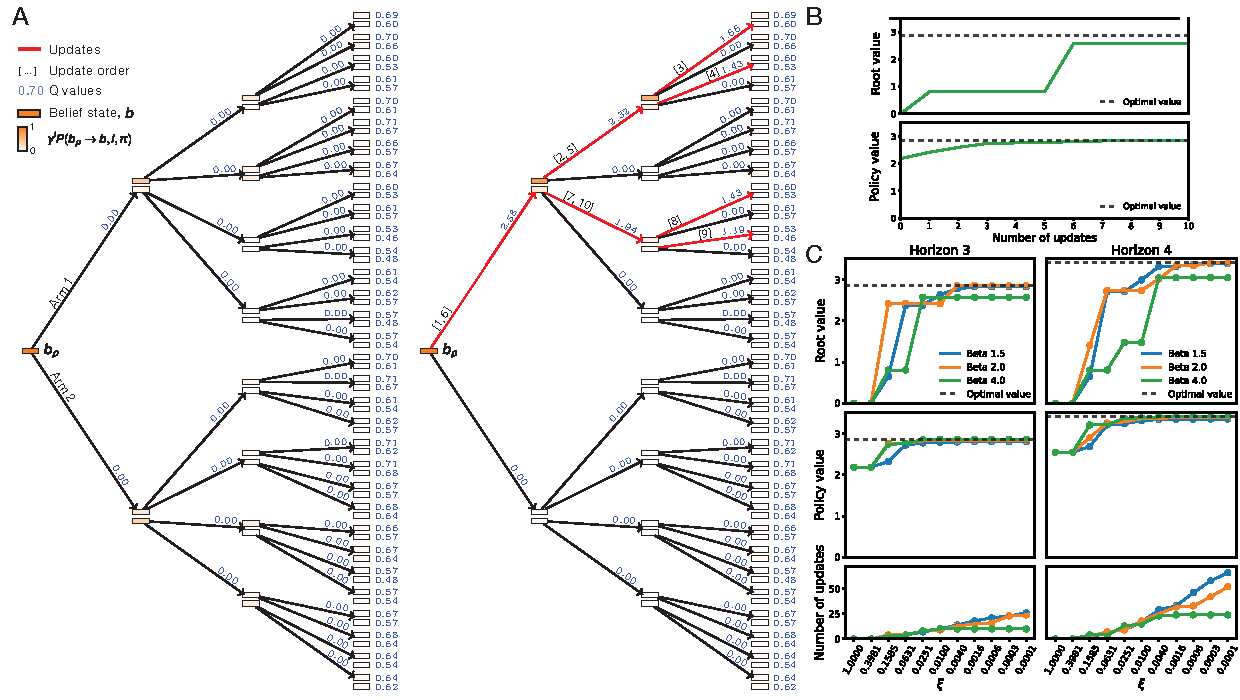
\includegraphics[width=1\textwidth]{Figures/fig1.png}
    \caption{\footnotesize \textbf{Exploitative replay can result in suboptimal behaviour.} A) Normalised state occupancy of the subject during first 2000 moves of exploration and learning in the environment. The start state is located at the bottom and the goal state is shown with the yellow clover. Note that all states were visited by the subject, including those besides the barriers (shown with opaque blue lines). B) Normalised maximal Gain that the subject estimated for the replay of each action (depicted with triangles), averaged across all 2000 moves. We only show actions for which the Gain was estimated to be positive. The actions which the subject would replay yielded a more exploitative policy which helped the subject acquire reward at a higher rate. C) Normalised maximal Need for each state that the subject estimated, also averaged over those same 2000 moves. All values were additionally averaged over 10 simulations. D-F) Same as (A-C) but for additional 2000 moves during which the top barrier was removed. Note that the estimated Gain did not change. Moreover, the state occupancy profile in D), as well as the estimated Need in F) highlight how the subject's behaviour reduced to pure exploitation. Because of the environmental change, however, this behaviour was rendered suboptimal due to the existence of a shorter path  that the subject  did not discover.}
    \label{fig:fig1}
\end{figure}

There are two coarse flavours of exploration: undirected and directed \parencite{wilsonBalancingExplorationExploitation2021}, along with many heuristic and approximate versions of the latter. Undirected exploration comes from introducing stochasticity into choice. Although sometimes effective \parencite{dawCorticalSubstratesExploratory2006}, it is typically suboptimal. Rather, exploration should be directed to reducing the uncertainty about which actions in the environment are ultimately best \parencite{feldbaumDualControlTheory1965}.  One standard heuristic \parencite{suttonDynaIntegratedArchitecture1991} (see also \parencite{agrawalTemporalDynamicsOpportunity2020}) is to add a form of notional exploration bonus to the outcome of  actions whose consequences are uncertain.\cut{, which assumes that uncertainty grows with the time since the action was last attempted, and makes the exploration bonus follow suit (see also \parencite{agrawalTemporalDynamicsOpportunity2020}). }

Optimal exploration generates  bonuses by maintaining probabilistically-correct beliefs about the environment and accounting 
carefully for the immediate and longer term consequences of resolving the implied uncertainty  \parencite{gittinsBanditProcessesDynamic1979,duffQLearningBanditProblems1995}. This amounts to performing regular optimal control, but in what is known as a belief-state decision problem in which the physical state of the subject in the environment is augmented by the subject's beliefs about the environment (in our later spatial case, how likely it thinks barriers are to have been removed). Such careful accounting is radically computationally intractable, for instance because the space of all possible beliefs is continuous, implying that the optimal policy can be very complex. We show how exploratory forms of Gain and Need can generalize the use of replay to realize a limited version of this accounting offline.

Most studies of hippocampal replay  have  focused on  navigation tasks. We therefore sought to make testable predictions for exploratory replay in a rich spatial environment inspired by \textcite{tolmanCognitiveMapsRats1948} 
(and report in the supplement similar results on the simpler, theoretically more tractable, case of multi-arm bandit problems). Our maze comprises three corridors which merge onto the common stem leading to the goal location (Fig~\ref{fig:fig1}). Those corridors differ in length, and thus an optimal reward-maximising agent (and rats \parencite{tolmanCognitiveMapsRats1948}) would prefer the shortest corridor. However, either just the shortest, or all but the longest, path might possibly be blocked by barriers. The accompanying uncertainty provides the motivation for exploration. 

\begin{figure}[h!]
    \centering
    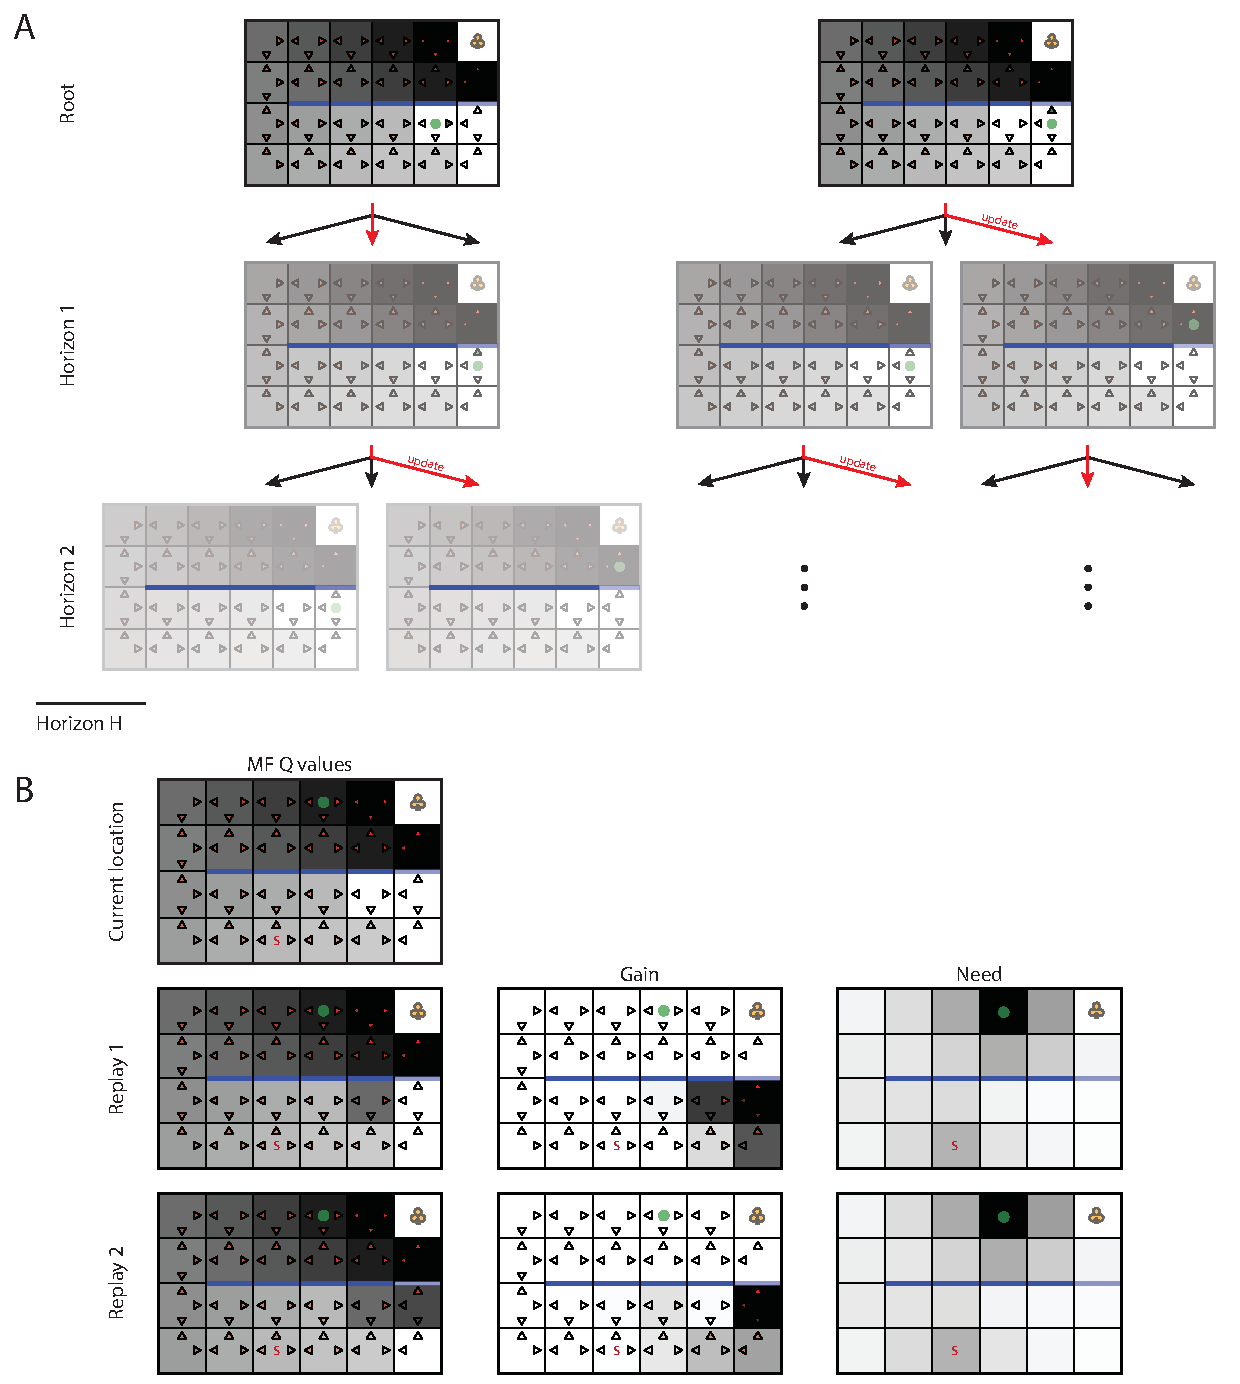
\includegraphics[width=1\textwidth]{Figures/fig2.png}
    \caption{\footnotesize \textbf{Exploratory replay leads to online discoveries, but potentially inadequate promulgation.} A) Prior state of knowledge of the subject. The intensity of the colour of each action arrow shows the respective model-free $Q$-values. Collectively, the action values represent the subject's model-free behavioural policy (i.e., the subject is more likely to choose actions with higher estimated $Q$-values -- those are highlighted with yellow outlines). Similarly, the states are coloured according to the maximal model-free $Q$-value at each state (which corresponds to state values). The inset next to the top barrier indicates the subject's prior belief about its presence (for the other barrier, the subject was certain that the path was blocked). The red dotted line shows the expected probability that the barrier is absent. The subject itself (green dot) is located at the start state. The goal state with reward is denoted with the yellow clover. B) Changes in the subject's model-free policy occasioned by exploratory replay updates. The numbers next to each action arrow indicate the order in which the replay updates were executed. C) New model-free policy which resulted from exploratory replay updates in B). Note how the action values now indicate that the subject should go towards the upper barrier. D) After pursuing the exploratory policy, the subject attempted to cross the top barrier; unfortunately, the barrier was found to be present -- this is indicated by both the subject's model-free $Q$-value associated with that action which was learnt online, as well as its new belief. E-F) Same as in B-C) but after the online discovery of the present barrier in D). The first replay choice of the subject correctly propagated the negative value of the present barrier to the immediately preceding state. However, as opposed to propagating this information deeper towards the start state, and hence correcting the exploratory policy in the light of the new information, the next replay choice of the subject made it more likely to visit an adjacent state which still contained the previously propagated exploration bonus, and hence had an erroneously (given the subject's new knowledge) high value.}
    \label{fig:fig2}
\end{figure}

For exploratory Gain: suppose that the subject is at a physical location just next to a barrier and is contemplating the action that might cross over and get close to the goal. To the extent the agent is uncertain that the barrier is 
absent, the action will fail, leading  to the belief that the barrier is there, and no Gain. However, as much as the agent is uncertain that the barrier is present, this action will succeed, leaving the subject in a new location, and with a new belief that the barrier is absent. This imagined outcome is associated with high Gain, because of the
implied shortcut estimated, in our account, based on the high model-free values for the new location. 

However, exploratory Need suffers from a chicken-and-egg problem in that if the          
subject adopts the purely exploitative policy of the known-to-be-open           
longest path, then the Need for the potential shortcut transition is            
zero (as the state next to the barrier is not visited). For simplicity, we make the approximation of including  stochasticity in the subject's behavioural policy (for instance, in the form of undirected exploration) such that Need is strictly positive for all possible belief states. This is achieved through applying a softmax behavioural policy \parencite{dawCorticalSubstratesExploratory2006}. 

The calculations of exploratory Gain and Need differ crucially from \textcite{mattarPrioritizedMemoryAccess2018} in terms of generalization. Individual physical locations (such as those next to barriers) can be visited with different beliefs about the environment. Importantly, discovering that a barrier is present/absent is information for all belief states associated with that barrier. This requires the subject to generalise the benefit of potential discoveries across multiple belief states.

As mentioned earlier, optimally accounting for the evolution of the subject's beliefs is woefully intractable. We therefore incorporated a form of second-order certainty equivalence approximation \parencite{dayanExplorationBonusesDual1996} for the estimation of exploratory Need. The subject optimally tracks how its belief will evolve up to a limited planning horizon beyond which the residual uncertainty remains fixed. This means that the subject still maintains its subjective uncertainty about the possible futures (unlike  conventional forms of certainty equivalence \parencite{cozzolinoMarkovianDecisionProcesses1965}); however, it assumes that no new knowledge can be acquired or environmental changes take place beyond its planning horizon.

We simulated behaviour in the Tolman maze and examined the replay patterns  produced as a result of  uncertainty about the presence of the upper barrier (Fig~\ref{fig:fig2}). Note that the subject has to choose which arm to pursue at a decision point remote from the potential barrier location. There is thus substantial cost for exploration: the subject
has to have sufficient belief that the barrier is open  -- otherwise the potential benefit of exploration (discovering a shortcut) would not exceed the cost of deviating from the current behavioural policy (current reward rate) \parencite{nivTonicDopamineOpportunity2007}.

\begin{figure}[h!]
    \centering
    \includegraphics[width=1\textwidth]{Figures/fig3.png}
    \caption{\footnotesize \textbf{Sequence replay helps deep value propagation.} The layout of the figure is the same as in Fig~\ref{fig:fig2}. A-C) Show the subject's initial and uncertain state of knowledge, changes to the online behavioural policy occasioned by exploratory replay, and the new updated exploratory policy due to such replay, respectively. The crucial difference being that the replay in B) was \cut{backward arrows along the green line} a sequence event -- i.e., the whole chain of actions was updated simultaneously (the actions which were updated in the replayed sequence are linked by a green line). D-F) Again, the subject discovered the top barrier, learnt about its presence online and engaged in replay to recompile its model-free behavioural policy in the light of the negative information. Note how, in this case, sequence replay in E) resulted in deep propagation of the value of such information all the way towards the start state. The sequence replay thus enabled the subject to  correct its exploratory policy appropriately.}
    \label{fig:fig3}
\end{figure}

Here, the subject's uncertainty resulted in consecutive replay updates which originated at the potential barrier location and progressed towards the subject's location in a reverse manner (Fig~\ref{fig:fig2}A-C). Those replays propagated the value of exploring the barrier towards the subject's current location, and the resulting new model-free behavioural policy indicated exploration was worthwhile (Fig~\ref{fig:fig2}C). As just discussed, the extent to which the subject was uncertain determined how large was the exploratory bonus that reached the subject's current state -- and thus produced policies with different incentives for exploration \toga{should fig S5 have single-action replay updates instead? since we only talk about sequence replay later}(Figs~\ref{fig:supp5} and~\ref{fig:supp6}). 

Resolving uncertainty can often result in unfortunate outcomes, for instance if the barrier is found actually to be present (Fig~\ref{fig:fig2}D). If this happens, it is important for the subject to  correct the full exploratory policy that had led to the discovery in the light of the negative information it acquired. We find that in our simulated Tolman maze, single-action replay updates do not handle this appropriately: the discovered value of the present barrier does not propagate deeply enough towards those states which had been updated with the exploratory bonus of the obsolete belief (Fig~\ref{fig:fig2}E-F). This is because  single-action updates are myopic: the estimated benefit of a single-action update does not account for how that update can affect the benefit of potential future updates. This problem does not arise if the shortcut is found to be available, since then the subject can efficiently exploit its new policy.

One plausible solution is to consider the benefit of simultaneously updating a sequence of actions, as opposed to  relying solely on updates at single states. This benefit combines Gain, that accumulates with the propagated policy changes (provided that all those changes result in policy improvements), as well as Need along that sequence of actions. We found that sequence replay results in deep propagation of the value of a discovered barrier, along the whole chain of actions which had previously been endowed with the exploration bonus (Fig~\ref{fig:fig3}).

Experimental evidence implicates the hippocampus in constructing replay sequences through previously unexplored spaces \parencite{guptaHippocampalReplayNot2010, olafsdottirHippocampalPlaceCells2015}. In our account, this corresponds to replay in potential future belief states which the subject has not visited yet but imagines to encounter. We manipulated the barrier configuration in our maze to produce a corridor segment in the central arm with both sides occluded by barriers (Fig~\ref{fig:fig4}). Examining the replay patterns chosen by the subject due to its uncertainty about the presence of both barriers revealed sequence replay in the corridor. Such replay propagated the exploratory value of learning about the possibility of entering the corridor (resolving uncertainty about the bottom barrier), exiting it (learning about the top barrier) and ending up in a state close to the goal.

\begin{figure}[h!]
    \centering
    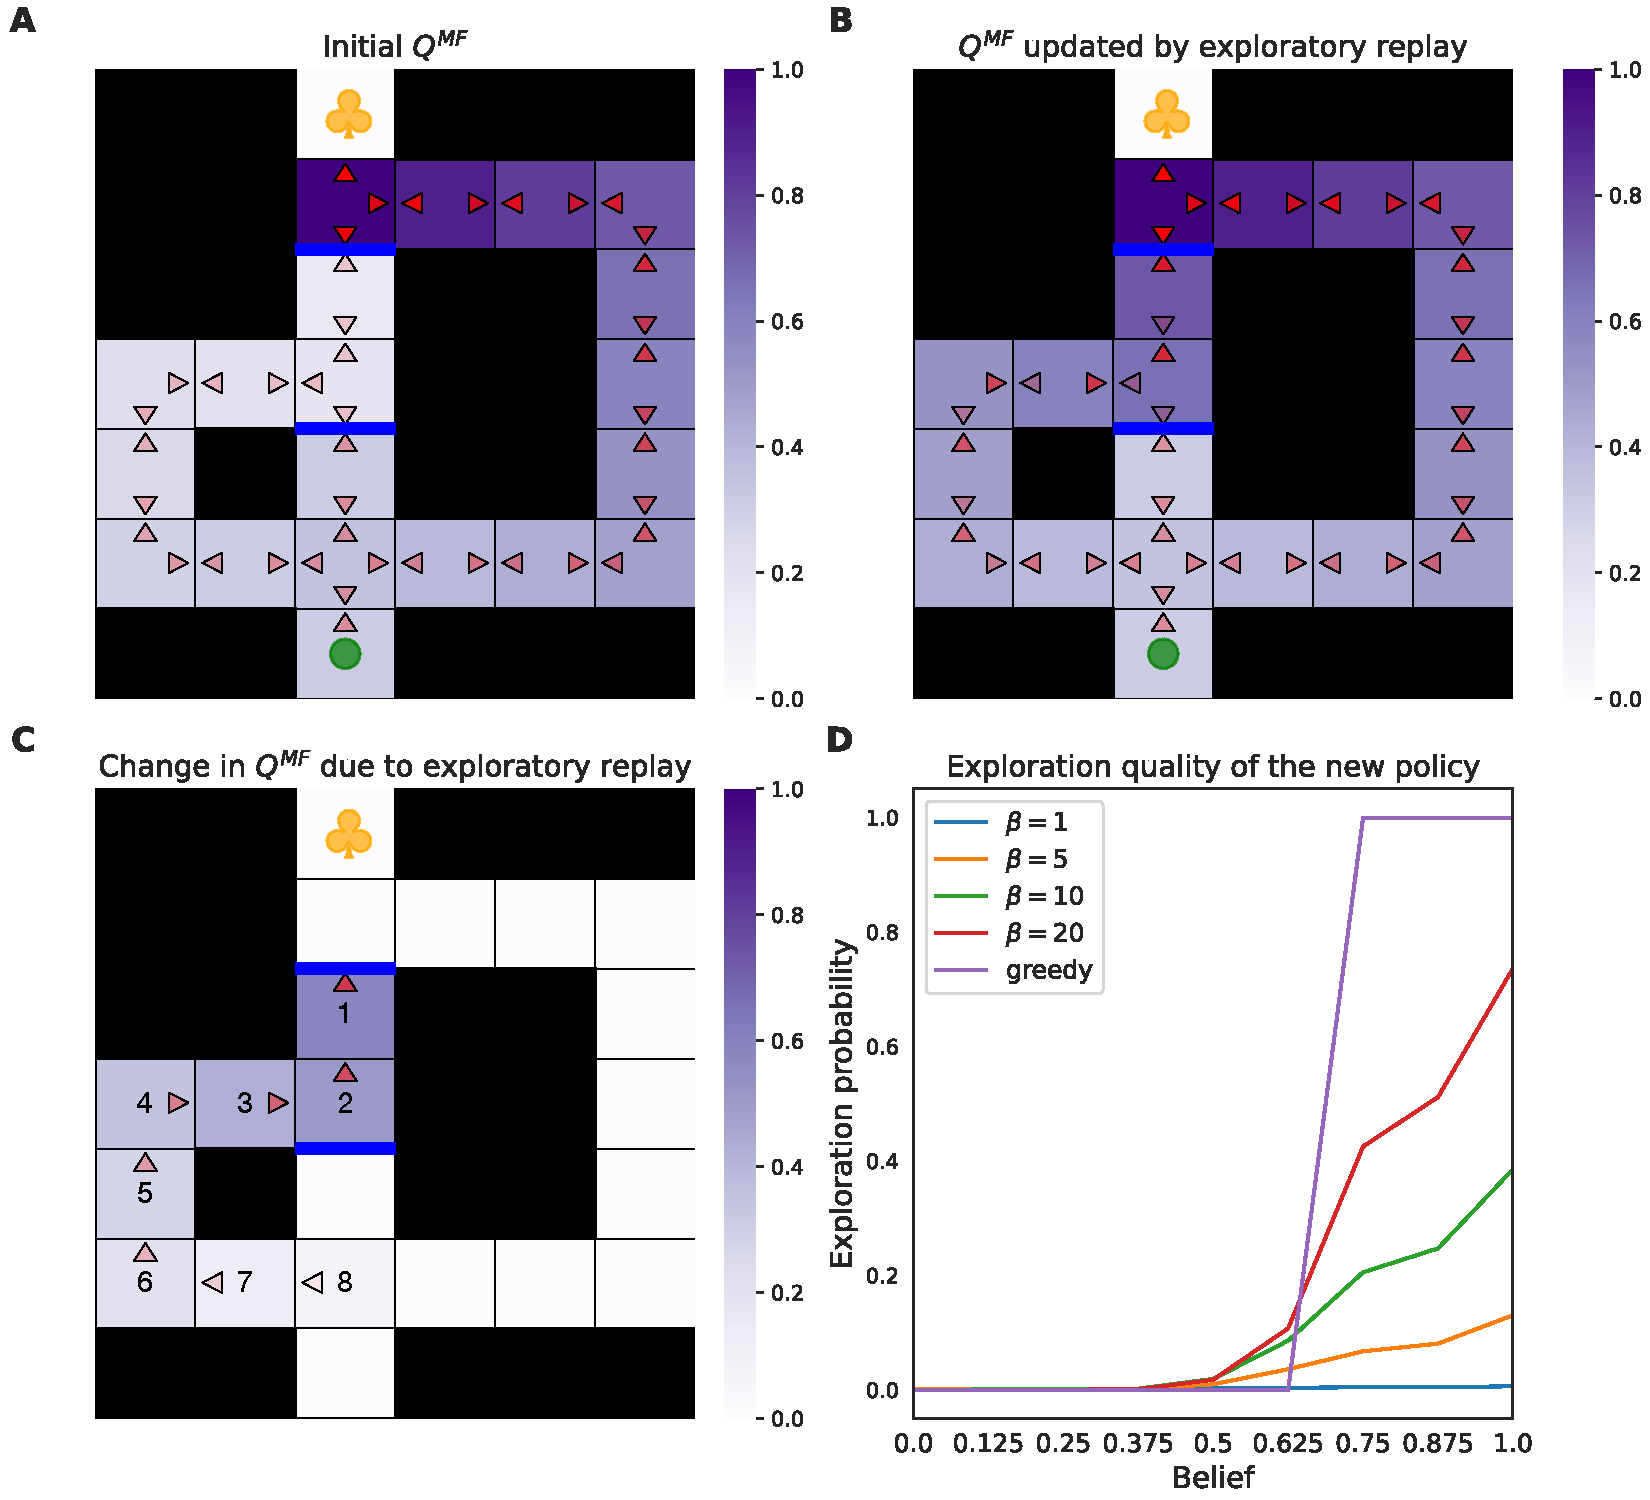
\includegraphics[width=1\textwidth]{Figures/fig4.png}
    \caption{\footnotesize \textbf{Replay in a blocked corridor.} A) Initial state of knowledge of the subject. Note that the model-free $Q$-values in the blocked corridor are all initialised to $0$, thus mimicking the subject's inexperience with the segment. The subject's belief state comprises its uncertainty about the presence of the top and bottom barriers that create the corridor. B) Replay choices of the subject due to its initial and uncertain state of knowledge. Note that replays inside the corridor correspond to a different belief state since they follow the potential transition through the bottom barrier which the subject has to first learn about. C) New exploratory policy occasioned by the replay updates in B).}
    \label{fig:fig4}
\end{figure}

Some of the most important facets of learning in the brain involve building inverse models: this characterizes bottom-up, recognition, models of sensory processing in cortex; the maintenance and expansion of the relationship between cortical and hippocampal representations in memory; and the determination of policies that maximize reward and minimize punishment given information about the environment. Offline processing, evident in replay, offers a way of building and refining inverse models of all these forms without disturbing ongoing behaviour. However, to determine good policies, it is not enough to build an inverse model based on just current information; active observers have the obligation to collect new information too, and balance this against exploitation. This obligation can be satisfied by inverting a more sophisticated model of the environment that includes uncertainty; here, we showed how to conceive of (reverse) replay as performing this inverse. This provided new insights into the nature and structure of offline activity -- for instance surfacing the importance of sequence replay, as well as predictions for new experimental paradigms.



\section{Methods}
We treated the (navigational) decision-making problem in our variant of the Tolman maze as a partially observable Markov Decision Process (POMDP). The subject was designed in the spirit of the DYNA architecture, such that online decisions were made according to the behavioural model-free policy, and offline planning was used to additionally train the model-free controller. The subject was endowed with a probabilistic belief about the existence of barriers in certain locations in the maze; every decision (real or imagined) therefore transitioned the subject to a new belief state which comprised the subject's physical state, as well as its updated prior belief. For planning (replay), the subject considered how its belief state will evolve up to a fixed horizon. The value of each imagined belief state was approximated with the subject's model-free $Q$-values at the corresponding physical location. Moreover, we discretised the possible belief states into the subject's initial uncertainty, and whether the barrier was certainly present or certainly absent. The priority of each replay update was determined by the expected long-run improvement to the subject's current belief state engendered by each potential replay update. The replay updates were executed until the expected improvement was estimated to be below a fixed threshold. For sequence replay updates, the maximal length of each potential sequence was limited to the distance from the start state to the uncertain barrier.

\clearpage
\section{Supplementary information}
\renewcommand{\thefigure}{S\arabic{figure}} 
\setcounter{figure}{0}
\subsection*{Theory background}

\subsubsection*{Reinforcement learning}
In reinforcement learning (RL) \parencite{suttonReinforcementLearningIntroduction2018}, subjects learn to make appropriate decisions in order to maximize expected gains and minimize potential losses.  Learning proceeds through interaction with an environment which supplies a sparse learning signal. The environment is typically formalised as a Markov Decision Process (MDP), which is a tuple $\langle \mathcal{S}, \mathcal{A}, \mathcal{P}, \mathcal{R}, \gamma \rangle$ where $\mathcal{S}$ is the set of states, $\mathcal{A}$ is the set of actions available at each state, $\mathcal{P}: \mathcal{S} \times \mathcal{A} \times \mathcal{S} \rightarrow [0, 1]$ is the Markov transition kernel which specifies the transition probabilities between states given an action, $\mathcal{R}:\mathcal{S}\rightarrow \mathbb{R}$ is a bounded reward function which comprises the learning signal, and $\gamma \in [0, 1)$ is the discount factor which determines the appetitiveness of delayed rewards.

The subject's behaviour in an environment is governed by its policy,  $\pi:\mathcal{S} \times \mathcal{A} \rightarrow [0,1]$, which, for every state, outputs a probability distribution over the set of available actions. At each time step, the subject interacts with its environment and receives the reward signal. The (possibly infinite) discounted collection of rewards the subject accrues along a trajectory of decisions is called the return. One main goal for a reinforcement learning subject
is  to predict the expected rewarding consequences of following  policy $\pi$ starting at a state $s$. This can be written as
\begin{equation}
    V^{\pi}(s) = \mathbb{E}_{\pi}\left[ \sum_{t=0}^{\infty} \gamma^t \mathcal{R}_t \mid S_0 = s \right]
    \label{eqn:value}
\end{equation}
A closely related task is instead to estimate the expected return for performing some action $a$ in a given state $s$, in which case they are referred to as  $Q$-functions:
\begin{equation}
    Q^\pi(s, a) = \mathbb{E}_{\pi}\left[ \sum_{t=0}^{\infty} \gamma^t \mathcal{R}_t \mid S_0 = s, A_0 = a \right]
    \label{eqn:qvalue}
\end{equation}

The second main goal is to learn an optimal policy, $\pi^*$, which for any starting state $s$ prescribes how to maximise the expected return: 
\begin{equation}
    \pi^* = \max_{\pi} \mathbb{E}_{\pi}\left[ \sum_{t=0}^{\infty} \gamma^t \mathcal{R}_t \mid S_0 = s \right]
\end{equation}
An MDP need not have a unique optimal policy. However, the optimal value function $V^{\pi^*}(s)$ and $Q^{\pi^*}(s,a)$ functions are unique. In particular, any action $a=\text{argmax}_{a'\in \mathcal{A}}Q^{\pi^*}(s,a')$ can be chosen.

\subsubsection*{Model-free control}

Several algorithmic approaches exist to solving the problem of optimal control in RL tasks. One popular
example is $Q$-learning \parencite{watkinsQlearning1992a}, which is an important and widely used algorithm for learning the optimal $Q^{\pi^*}$-function. It belongs to a more general class of model-free temporal difference algorithms which, after every experienced interaction with the environment, successively update their value function estimates based on the encountered reward prediction errors. Specifically for $Q$-learning, the update rule at iteration $n$ is:

\begin{equation}
    Q^{n+1}(s, a) \leftarrow Q^{n}(s, a) + \alpha \left[\mathcal{R}(s') + \gamma \max_{a'\in\mathcal{A}} Q^{n}(s', a') - Q^{n}(s, a)\right]
    \label{eqn:qlearning}
\end{equation}

Here, the $Q$-value estimate is updated towards the difference (or prediction error) between the initial estimate, $Q^{n}(s, a)$, and the sum of the observed reward at the next state reached and the discounted maximal $Q^{n}$-value at that state, $\mathcal{R}(s') + \gamma \max_{a' \in \mathcal{A}}Q^{n}(s', a')$, weighted by the learning rate, $\alpha$. Note that the action that optimises $Q^{n+1}(s, a')$ at $s$ might be different from the one used in equation~\ref{eqn:qlearning} that optimized $Q^n(s, a')$

The $Q^{n+1}$-values themselves can be used to determine a  policy, for instance:
\begin{equation}
    \pi^{n+1}(s,a)=\frac{e^{\beta Q^{n+1}(s, a)}}{\sum_{a'\in\mathcal{A}} e^{\beta Q^{n+1}(s, a')}}
  \end{equation}
where $\beta>0$ is an inverse temperature parameter that controls how deterministic is $\pi^{n+1}$. Since $\pi^{n+1}(s,a)$ favours actions with higher $Q^{n+1}$-values, it tends to be better than $\pi^n(s,a)$ in terms of expected return. The remaining stochasticity is a crude method for arranging a mix of exploration and exploitation.

\cut{
The subject's behaviour (policy) is then fully specified by the set of learnt value functions. In the case of a deterministic policy (which is a special case of a broader class of stochastic policies), for example, the subject would always choose actions with highest estimated $Q$-values. This is, in fact, what makes model-free control \emph{fast}: making decisions does not consume time since for every state of the environment it only involves picking an action based on the cached values learnt online. When it comes to environmental changes, however, model-free control is rather stubborn and inflexible since it requires direct experience with the environment to propagate the long-run effects of those changes to distal actions. }

\subsubsection*{Model-based control}

A different solution is to learn a model of the environment which can then be used to perform prospective \emph{planning} of the actions to execute. Value functions can also be acquired using the recurrent Bellman equation \parencite{bellmanTheoryDynamicProgramming1954}, for instance:

\begin{equation}
    Q^{n+1}(s, a) =  \sum_{s'}\mathcal{P}(s'\mid s, a)\left[\mathcal{R}(s') + \gamma \max_{a'\in\mathcal{A}} Q^{n}(s', a') \right]
    \label{eqn:bellman}
\end{equation}

Here, the recurrent relationship between the successive states allows the subject to make use of its knowledge of the transition structure of the environment (the model $\mathcal{P}$) to propagate the information about future rewards towards its current situation or state in the environment. If the subject does indeed know the model (also including $\mathcal{R}$), then various forms of planning can be used to compute the long-run consequences associated with the available actions at decision time and make a far-sighted and informed decision. Value iteration \parencite{bellmanTheoryDynamicProgramming1954} is one example planning algorithm which iteratively performs synchronous updates (for all states and actions in each sweep) specified by Equation~\ref{eqn:bellman}. Such updates are also called Bellman backups because of the application of the Bellman equation. Given a perfect model of the environment, $\mathcal{P}$, such procedure is guaranteed eventually to  converge to the optimal value function.

\cut{
Model-based planning has its own perils and merits: it is \emph{slow} since the action values have to be computed from scratch; however, it enables behavioural flexibility because once a change in the environment is discovered, this knowledge can be immediately incorporated into the model and action values recomputed.}

\subsubsection*{DYNA and prioritized sweeping}

There is evidence for the use in animals, and the utility in artificial agents, of both model-free and model-based control \parencite{glascherStatesRewardsDissociable2010}. This poses obvious questions about their arbitration and integration \parencite{dawUncertaintybasedCompetitionPrefrontal2005, antonovOptimismPessimismOptimised2022, agrawalTemporalDynamicsOpportunity2020}. One important suggestion for integration is that information could be transferred from the model that the model-based controller possesses into the model-free controller, so that the latter can provide better informed choices.

In RL, the most common version of this process is known as experience replay \parencite{linSelfimprovingReactiveAgents1992}, and lies at the heart of many successful algorithms \parencite{schaulPrioritizedExperienceReplay2016}. Although, as we will discuss later, it was originally designed for the purpose of exploration, the so-called DYNA algorithm \parencite{suttonDynaIntegratedArchitecture1991} has been used to underpin this process. In DYNA, an agent  learns model-free value functions online by direct experience with the environment, as well as learning the model of that environment. During offline states, DYNA uses its learnt model to sample possible transitions and rewards, which are then used to perform further training of  the model-free value functions to perform a more effective form of model inversion.

Given this overall structure, it becomes natural to consider which transitions or rewards should be sampled from the model (or replayed). One important algorithmic notion is prioritized sweeping \parencite{moorePrioritizedSweepingReinforcement1993}, in which replays are chosen in an order that effects a form of optimal improvement in the model-free value functions.


\subsubsection*{Gain and Need}

\textcite{mattarPrioritizedMemoryAccess2018} synthesised the ideas of DYNA and prioritised sweeping and proposed a principled, normative scheme for the ordering of planning computations. They suggested that each replay experience corresponds to a Bellman backup (Equation~\ref{eqn:bellman}) which uses information from a generative model of the environment to update a specific model-free state-action value.

\textcite{mattarPrioritizedMemoryAccess2018} observed that what is important about an update at a state (which could be distal from the current state of the agent) is whether it changes the subject's behavioural policy. For example, performing a planning computation at state $s_k$ corresponds to changing the model-free value for action $a_k$ at that state. Such a change is significant if the agent's behavioural policy changes at $s_k$; the agent can then estimate the consequence of that change for the expected return from its current state or a start state. 

\cut{
When the subject is located at some state $s$, its model-free value at that state, $V^\pi(s)$, indicates how much reward it expects to obtain from that state onwards by acting according to its current behavioural policy, $\pi$. The subject can decide to act, if content with the reward it expects; or the subject can plan to potentially improve its behavioural policy in the hope of obtaining higher reward.}

\textcite{mattarPrioritizedMemoryAccess2018} showed that the subject can calculate how a replay update to action $a_k$ at state $s_k$ changes the amount of reward it can obtain in the future starting from a potentially different  state $s$. By decomposing the difference in the subject's model-free value function estimate before and after the policy update occasioned by such replay update, $V^{\pi_{\text{new}}}(s)-V^{\pi_{\text{old}}}(s)$, \textcite{mattarPrioritizedMemoryAccess2018} showed that this expression can be written as:

\begin{equation}
    V^{\pi_{\text{new}}}(s)-V^{\pi_{\text{old}}}(s) = \sum_{x\in \mathcal{S}}\sum_{i=0}^{\infty} \gamma^i P(s\rightarrow x, i, \pi_{\text{old}}) \times \sum_{a} \left[\pi_{\text{new}}(a\mid x) - \pi_{\text{old}}(a\mid x) \right] Q^{\pi_{\text{old}}}(x, a)
    \label{eqn:evb_full}
\end{equation}
Furthermore, by assuming that each individual replay update to the model-free value of action $a_k$ results in a policy change at a single update location, $s_k$,  equation~\ref{eqn:evb_full} can be simplified into the product of Gain and Need, which \textcite{mattarPrioritizedMemoryAccess2018} termed the expected value of a backup ($\text{EVB}_{\pi_{\text{old}}}$):
\begin{equation}
    \text{EVB}_{\pi_{\text{old}}}(s_k, a_k) = \underbrace{\sum_{i=0}^{\infty} \gamma^i P(s\rightarrow s_k, i, \pi_{\text{old}})}_{\text{Need}} \times \underbrace{\sum_{a} \left[\pi_{\text{new}}(a\mid s_k) - \pi_{\text{old}}(a\mid s_k) \right] Q^{\pi_{\text{old}}}(s_k, a)}_{\text{Gain}}
    \label{eqn:evb_short}
\end{equation}

Gain quantifies the expected local improvement in the subject's behavioural policy at state $s_k$ as a result of the replay update. Thus, Gain is higher for those replay updates which result in greater policy changes at the update state. Need, on the other hand, quantifies how likely is the subject to visit the update state in the long run, given its model of the environmental transition dynamics and behavioural policy before the update.

In rodents, the hippocampus is a structure known to be involved in aspects of model-based control \parencite{pfeifferHippocampalPlacecellSequences2013, ambroseReverseReplayHippocampal2016, cazeHippocampalReplaysScrutiny2018}. \textcite{mattarPrioritizedMemoryAccess2018} suggested that the reactivation of sequences of behaviourally-relevant experiences during quiet wakefulness and sleep for which the hippocampus is well known \parencite{fosterReplayComesAge2017} is an expression of this sort of prioritized replay. They thereby explained a wealth of experimental findings on the selection of replay experiences in rodents \parencite{ambroseReverseReplayHippocampal2016, pfeifferHippocampalPlacecellSequences2013} as well as humans \parencite{liuPrioritizedExperienceReplay2022, antonovOptimismPessimismOptimised2022}. 

\subsubsection*{Exploration}

As discussed in the main text, exploration in MDPs can be accomplished by the use of heuristics which estimate the amount of the subject's (in)experience with its environment. One such celebrated heuristic is based on the 'optimism in the face of uncertainty' (OFU) principle which posits that actions whose outcomes are uncertain should receive a sort of exploration bonus which would encourage the subject to pursue them. \textcite{suttonDynaIntegratedArchitecture1991}'s exploration bonus indeed took that form:

\begin{equation}
    Q^{n+1}(s,a) \leftarrow Q^n(s,a) + \alpha \left[ \mathcal{R}(s') + \epsilon \sqrt{\#_{(s,a)}} + \gamma \max_{a'\in\mathcal{A}}Q^n(s',a') - Q^n(s,a) \right]
    \label{eqn:bonus}
\end{equation}

Improved exploration in DYNA (also known as DYNA-$Q+$) was achieved by updating its model-free $Q$-values according to Equation~\ref{eqn:bonus} during offline planning. Here, $\#_{(s,a)}$ is a count-based heuristic which grows with the number of time steps since that state-action pair had last been attempted, and $\epsilon$ is a free parameter which controls the amount of influence this uncertainty bonus has on the $Q$-value update. By using this update rule, actions which have not been tried for an extended period of time come to look more appealing, which happens to be particularly useful in dynamic environments with unsignalled changes.

Note that by virtue of the $Q$-learning update rule (Equation~\ref{eqn:qlearning}), the exploration bonus awarded to a distal state-action pair (Equation~\ref{eqn:bonus}) propagates towards state-actions which lead to it, hence encouraging off-policy exploration. The bonus itself, however, is myopic, since it does not reflect the benefit of learning about the uncertain state-action in the first place. 

Optimal exploration, on the other hand, entails a more careful evaluation of how resolving one's uncertainty may be useful in the long-run and whether the acquired knowledge would be of any use for subsequent exploitation. Such thorough evaluation requires the subject to maintain an explicit model of its uncertainty and what possibilities abound.

\subsubsection*{Partial observability}

The classical MDP formalism assumes that the subject knows the model of the environment with which it interacts. It does not, however, capture the ignorance that subjects (at least partially) face when learning about their environments. Such ignorance can be treated as a form of incomplete information which the subject can (at least to some extent) complete with experience.

Partially observable Markov Decision Processes (POMDPs) are a generalisation of MDPs in which the subject can lack direct access to some knowledge that is required to learn a good policy. For instance, the subject can be ignorant about the state it occupies because instead of perfect information from the environment it receives noisy and ambiguous observations; alternatively, the subject can be uncertain about the transition dynamics that govern its movement through the environment.

Each observation in a POMDP therefore grants the subject a  piece of information which it can use to optimally update its knowledge about the environment. A sequence of observations the subject collects is formally referred to as \emph{history}. Critically, the subject's policy in a POMDP depends on its full history of observations, since this history determines its state of knowledge about the environment, and thereby determines the decisions it ought to make. The dependence on history violates the Markovian assumption (which requires that future transitions and rewards are statistically independent of the history, given the present state), and POMDPs are therefore not amenable to classical MDP solutions. 

Instead of keeping track of all encountered observations the subject can maintain a sufficient statistic of the entire history. This sufficient statistic is called the subject's \emph{belief}, and it concisely summarises the knowledge that the subject has acquired. With each new observation the subject can optimally update its beliefs in the light of new information. Beliefs can be viewed as a new, subjective, state for a decision problem; they do satisfy the Markov property, and so it is possible to formulate POMDPs as MDPs where each state of the process is the subject's belief. 

A belief MDP is therefore formally defined as a tuple $\langle \mathcal{B}, \mathcal{A}, \mathcal{T}, \mathcal{R}, \gamma \rangle$ where $\mathcal{B}$ is the (continuous) set of belief states, $\mathcal{A}$ is the set of actions, $\mathcal{T}: \mathcal{B} \times \mathcal{A} \times \mathcal{B} \rightarrow [0,1]$ is the (Markov) belief transition kernel, $\mathcal{R}:\mathcal{B}\rightarrow \mathbb{R}$ is a bounded reward function, and $\gamma \in [0, 1)$ is the discount factor. Thus, as opposed to the original MDP formulation, in belief MDPs the subject transitions through augmented belief states. For our matters, each belief state, $b=\{ s \in \mathcal{S}, P(\mathcal{P}) \}$, encompasses the subject's physical location in the environment, $s$, as well as its probabilistic model of uncertainty, $P(\mathcal{P})$, about the presence/absence of barriers at several locations.

The formalism of belief MDPs permits the construction of policies which optimally trade-off exploration and exploitation \parencite{guezSampleBasedSearchMethods2015}. To see this, consider the case that the subject is uncertain about the state transition model $\mathcal{P}$, and therefore maintains a prior belief $P(\mathcal{P})$. Firstly, the probabilistic belief allows the subject to learn optimally upon receiving observations from the environment -- in the case of transition uncertainty, by noting which state each transition leads to. This is accomplished by calculating a posterior belief using Bayes' rule:

\begin{equation}
    P(\mathcal{P} \mid s) = \frac{P(s\mid \mathcal{P})P(\mathcal{P})}{\sum_{s' \in \mathcal{S}}P(s'\mid \mathcal{P})P(\mathcal{P})}
    \label{eqn:bupd}
\end{equation}

Secondly, the subject can plan the future possibilities by making use of its uncertainty and allocating the prior probabilities to each of the considered outcomes. Those outcomes, in turn, result in more potential learning which the subject also accounts for by performing the same updates as in Equation~\ref{eqn:bupd} but for simulated futures (those transitions are governed by the belief MDP transition function, $\mathcal{T}$). This allows the subject to foresee the long-run consequences associated with each exploratory decision and whether it can potentially result in better future return.

\subsection*{Model description}

\subsubsection*{Replay updates}

The subject makes use of its transition model as well as the associated uncertainty to envision the possible evolution of its belief. This can be visualised as a planning tree which is rooted at the subject's current belief state, $b_\rho$. The subject considers all possible actions from this root node, and adds additional nodes for each new belief state that results from applying those actions (according to the belief transition model, $\mathcal{T}$) -- this corresponds to adding a single step horizon to the planning tree. Applying the same procedure to all nodes at the new horizon further deepens the tree and expands the planning horizon.

Similarly to physical states in MDP problems, each belief state can have an associated value which reflects how much reward the subject expects to obtain by being in that belief state and acting according to some policy. Those values, however, are initially unknown to the subject, and the reason for performing replay updates in the belief tree is to propagate the value information from future belief states to the subject's current belief state. Since belief states are continuous, we restrict the subject's planning horizon to a fixed depth. This means that belief states containing reward may be beyond the subject's reach. However, the subject's model-free system is likely to have an estimate of how valuable each physical location is. Therefore, the model-based value of each action $a$ at every belief state $b = \{ s, P(\mathcal{P}) \}$ in the planning tree, which we refer to as $Q_{MB}^n(b, a)$, is initialised to the subject's model-free estimate of the value of performing this action at a physical location in that belief state, $Q_{MF}^0(s, a)$.

When performing replay updates, the subject considers the effect of each action at every belief state in the tree rooted at its current belief state. For example, when considering the effect of action $a$ at belief state $b = \{ s, P(\mathcal{P}) \}$ which attempts to cross a potential barrier, the subject accounts for the possibility of transitioning into one of two new belief states: $b'_{\text{open}} = \{ s', P'_{\text{open}}(\mathcal{P}) \}$, which corresponds to the fortunate outcome of discovering that the barrier is absent, and $b'_{\text{closed}} = \{ s, P'_{\text{closed}}(\mathcal{P}) \}$, which corresponds to the unlucky outcome of the barrier being present. This amounts to updating the value associated with executing action $a$ at belief state $b$ towards the expected value of the next belief states:

\begin{equation}
    Q_{MB}^{n+1}(b, a) = Q_{MB}^n(b, a) + \sum_{b' \in \{ b'_{\text{open}}, b'_{\text{closed}} \}} \mathcal{T}(b'\mid b, a)\left[ \mathcal{R}(b') + \gamma \max_{a'\in\mathcal{A}} Q_{MB}^n(b', a') - Q_{MB}^n(b, a) \right]
    \label{eqn:repupd}
\end{equation}
Here, the belief transition model, $\mathcal{T}$, describes how the subject jointly transitions through physical states and its beliefs about the barrier configuration, i.e. $\mathcal{T}(b'\mid b, a)=P(s', b'\mid s, a, b)$. Moreover, for brevity, we will refer to the set of belief states that the subject can reach by applying a single action at a belief state as the children set of that belief state, denoted as $C(b, a) \in \mathcal{B}$. For the example above: 

\begin{equation}
    C(b, a) = \{ b'_{\text{open}}, b'_{\text{closed}} \}
    \label{eqn:children}
\end{equation}

\subsubsection*{Gain and Need in belief space}
We consider optimising the prioritisation of replay updates (Equation~\ref{eqn:repupd}) in the subject's belief space. We follow the suggestion of \textcite{mattarPrioritizedMemoryAccess2018}, whereby the priority of each update is determined by the expected improvement to the subject's behaviour at its current belief state. By applying the same value decomposition as in \textcite{mattarPrioritizedMemoryAccess2018}, we define $\text{EVB}_{\pi_{\text{old}}}(b_k, a_k):=V^{\pi_\text{new}}(b_\rho) - V^{\pi_{\text{old}}}(b_\rho)$, where $V^{\pi_{\text{old}}}(b_\rho)$ is the value the subject estimates for its current belief state, $b_\rho$, under the old behavioural policy before the potential update, and $V^{\pi_\text{new}}(b_\rho)$ is the estimated value of the subject's current belief state under the new policy implied by the potential update. The effect of policy change engendered by a replay update to action $a_k$ at some (potentially distal) belief state $b_k$ can be expressed as:

\begin{equation}
    \text{EVB}_{\pi_{\text{old}}}(b_k, a_k) = \sum_{b\in \mathcal{B}} \underbrace{\sum_{i=0}^{\infty} \gamma^i \mathcal{T}(b_\rho \rightarrow b, i, \pi_{\text{old}})}_{\text{Need}} \times \underbrace{\sum_{a}\left[\pi_{\text{new}}(a\mid b) - \pi_{\text{old}}(a\mid b)\right]Q^{\pi_{\text{old}}}(b, a)}_{\text{Gain}}
    \label{eqn:evb}
\end{equation}

Importantly, we do not assume that the effects of replay updates are localised to individual states (as in Equation~\ref{eqn:evb_short}), which allows the subject to account for broad generalisation across multiple belief states (see below) when calculating the expected benefit of each replay update. The Gain term associated with a replay update quantifies the expected local improvement in the subject's behavioural policy at the update belief state engendered by that replay (Equation~\ref{eqn:repupd}). Gain therefore favours those replay updates which result in large improvements to the subject's model-free decision policy.

Need, similarly to \textcite{mattarPrioritizedMemoryAccess2018}, quantifies the frequency with which the subject expects to visit the update belief state according to its old behavioural policy, $\pi_{\text{old}}$. As discussed before, in belief MDPs, subjects engage in continual learning which means that with every visit to the same physical location the subject has a different belief about the transition model. This allows the belief space version of Need to account for all possible future learning that can take place (however, for computational purposes, we limit the subject's horizon -- see below).

One critical consideration is that of the dependence of Need on the old behavioural policy of the subject, $\pi_{\text{old}}$, which tends to prioritise portions of the state space the subject already expects to visit. Thus, even if the subject was informed about a distal change in the transition structure which its current policy does not prescribe to visit, Need at those locations would still be zero. It is therefore important to include stochasticity (for instance, in the form of undirected exploration) into the subject's behavioural policy which generates Need to allow for off-policy replay choices. This motivates our choice of the softmax behavioural policy which ensures that Need is positive for all potential belief states. Below we additionally explore how the subject's behavioural policy affects it replay choices. 

As for \textcite{mattarPrioritizedMemoryAccess2018}, we set a threshold on the minimal $\text{EVB}_{\pi_{\text{old}}}$ value required for an update to be executed. This threshold can be thought of as accounting for a form of opportunity cost by balancing the trade-off between planning to improve the policy and immediately acting to collect reward \parencite{nivTonicDopamineOpportunity2007}, hence helping to subject to avoid being permanently buried in thought.

\subsubsection*{Generalisation}
The notable difference between our belief space decomposition and that of \textcite{mattarPrioritizedMemoryAccess2018} is the inclusion of the outer sum over the space of beliefs, $\mathcal{B}$. This critical difference enables the subject to account for a broad generalisation across multiple belief states when considering the effect of a single action update at an individual belief state. 

Each belief state in continual learning tasks (unless there is forgetting) can be visited at most once since after every transition the subject potentially acquires information, and therefore updates its prior belief which constitutes a different belief state. However, even though each belief state can be visited at most once, physical states which also comprise those belief states reoccur in episodic tasks. The subject can therefore expect an accumulated benefit of replay updates at single belief states. Moreover, information that the subject discovers about a potential barrier (for instance, if it is absent) is shared across all belief states associated with that barrier -- since at any time it can only be present or absent. 

\subsubsection*{Sequence replay}

Sequence replay corresponds to updating a whole sequence of consecutive actions, as opposed to performing individual greedy action updates one at a time. For example, consider two consecutive actions $a_1$ and $a_2$ at belief states $b_1$ and $b_2$, respectively. The order in which those two replay updates are executed depends on the expected value associated with the two possibilities. In the spatial domain (or other domains with clear ordering) one order would typically be interpreted as a reverse reactivation, and the other as forward. Moreover, the expected value of performing forward and reverse sequence updates will, in general, differ (see below). A sequence update to the two example actions corresponds to updating one action according to:

\begin{equation}
    Q_{MB}^{n+\frac{1}{2}}(b_1, a_1) = Q_{MB}^n(b_1, a_1) + \sum_{b' \in C(b_1, a_1)} \mathcal{T}(b'\mid b_1, a_1)\left[ \mathcal{R}(b') + \gamma \max_{a'\in\mathcal{A}} Q_{MB}^n(b', a') - Q_{MB}^n(b_1, a_1) \right]
\end{equation}
where the sum is over the set of next possible beliefs (as in equation ~\ref{eqn:children}). The fractional notation $n+\frac{1}{2}$ emphasises the fact that within a single iteration of replay multiple actions can simultaneously be replayed in a sequence, since in the current example with two actions there are two executed updates between iterations $n$ and $n+1$.

The second action is then updated in the same way to generate $Q_{MB}$; however, in the case of reverse replay, $b_1 \in C(b_2, a_2)$, and therefore the $Q_{MB}^{n+\frac{1}{2}}$-value of one of its children beliefs $b'\in C(b_2, a_2)$ will have already been updated. The size of the value update to action $a_2$ at belief state $b_2$ therefore depends on the update to action $a_1$ at belief state $b_1$. This is also reflected in how the expected value of sequence replay is calculated -- which is the reason for why the benefit of sequence replay can be larger than that of single action updates. If we define $\mathcal{M}_N=\{ (b, a)_{i} \}_{1, ..., N}$ as the candidate set containing $N$ belief state-action pairs to be potentially updated in a sequence replay event, then the expected benefit of that sequence replay is calculated as:

\begin{equation}
    \text{EVB}_{\pi_{\text{old}}}(\mathcal{M}_{N}) = \sum_{(b, a) \in \mathcal{M}_N} \text{EVB}_{\pi_{\text{old}}}^{n+\frac{1}{N}}(b, a)
    \label{eqn:evbseq}
\end{equation}

Note that, in the case of reverse replay, each individual $\text{EVB}_{\pi_{\text{old}}}(b, a)$ in Equation~\ref{eqn:evbseq} quantifies the benefit of updating action $a$ at belief state $b$ with a value that is propagated towards it along the sequence of actions that had also been updated. This is not the case for forward replay where each action is updated only towards the expected value of its children belief states; however, even in the case of forward replay the benefit of replaying the whole sequence will still, in general, be higher because of the summed benefit of all updates along the entire sequence (see below).

Replayed sequences can be of arbitrary lengths. Moreover, the longer the sequence, the more the estimated expected benefit will be, in general. The natural question therefore arises concerning the termination of sequences. We do not address this issue in the current work and assume that sequences link together critical decision points -- in the Tolman maze, for instance, this corresponds to the sequential replay which originates at a potential barrier location and progresses towards the intersection in front of the subject's start state. 

Another consideration is computational: the theory that \textcite{mattarPrioritizedMemoryAccess2018} proposed is normative and does not prescribe how both Gain and Need can possibly be estimated in a psychologically credible way. Sequence replay is even more computationally prohibitive because of the number of potential sequences that can be replayed. In the present work, we similarly report a normative result describing which sequences (out of all possibilities up to a fixed length) should be replayed. How the brain manages to reduce the sample complexity of sequence replay thus remains an open and challenging question which we leave to future work.

\subsection*{Simplified example: Bayesian bandits}

Stationary, multi-arm bandit (MAB) problems offer the  simplest test bed for examining exploration in belief spaces, and we therefore provide simulation results of replay prioritisation in a class of MABs. A typical MAB problem consists of a finite set of $K$ arms, $\mathcal{A} = \{ a_1, ..., a_K \}$, which are the equivalent of actions in sequential decision-making problems. In each of the infinitely many trials, the subject is faced with a choice to pull one of the available arms. Each of the $K$ arms, say $a_k$, if chosen, has a certain probability, $\mu_k$, of paying  the subject off with a binary reward ($1$ with probability $\mu_k$ and $0$ with probability $1-\mu_k$). 

MAB problems are well-studied and, under certain assumptions about the reward distribution, optimal policies can be derived (such as the Gittins index \parencite{gittinsBanditProcessesDynamic1979}). Importantly, the payoff probabilities associated with each arm are initially unknown to the subject. This makes exploration in MAB problems worthwhile even if the expected return for the arm concerned is low, since if the arm is found actually to be good, then it can be consistently exploited in the future. Furthermore, MABs lack physical states, since in each trial the subject is faced with the same selection of arms irrespective of its choices in the preceding trials. The lack of physical states and the necessity of exploration makes MABs a perfect case study for our replay prioritisation, which we detail below. 

    We focus on a 2-arm bandit task with binary outcomes, in which on each trial, the subject has to choose between two arms, $a_1$ and $a_2$, which have unknown payoff probabilities, $\mu_1$ and $\mu_2$,  respectively. The subject models its uncertainty about the payoff probability of each arm with a probabilistic prior belief which introduces subjective belief states, $b=\{ p(\mu_1), p(\mu_2) \}$. Just as in the Tolman maze example considered above, a probabilistic model of uncertainty allows the subject to  learn optimally about the payoff distribution of each arm after receiving feedback from the bandit in the form of a reward signal. 

We model the subject's uncertainty about each arm's payoff probability using the Beta distribution. This particular parametric form is very convenient since the Beta distribution is a conjugate prior for the Bernoulli distribution (which is the reward distribution of each arm). The Beta distribution has two parameters, $\alpha$ and $\beta$, where $\alpha$ is typically interpreted as the number of success trials (received a reward of $1$) and $\beta$ as the number of failed trials (received a reward of $0$). After $N$ choices of arm $a_k$, the Bayesian update (Equation~\ref{eqn:bupd}) to the prior distribution parameters (i.e., the subject's belief state) due to a new observation corresponds to:

\begin{align}
    p(\mu_k \mid \mathcal{R}=r) = 
    \begin{cases}
    \text{Beta}(\alpha_N + 1, \beta_N), \; \text{if $r=1$}\\
    \text{Beta}(\alpha_N, \beta_N+1), \; \text{if $r=0$}
    \end{cases}
\end{align}

The subject can make use of its model of uncertainty to plan ahead how the choice of each arm will affect its belief. We visualise this as a planning tree in Fig~\ref{fig:supp1}A. The tree is rooted at the subject's current belief state, $b_\rho$, and each action (choosing arm $a_1$ or $a_2$) can transition the subject into two new possible belief states: one which corresponds to an imagined success trial and another corresponds to an imagined failure trial. Applying actions to belief states deepens the tree and expands the subject's planning horizon. The transition probabilities between successive belief states are governed by the belief transition model, $\mathcal{T}$. Note that the subject's planning horizon is limited to a fixed depth (Fig~\ref{fig:supp1}). This is because belief states are continuous, and building the entire tree of all possibilities is intractable. In our example, the subject therefore only considering how its belief will evolve up to several steps into the future.

Analogously to the Tolman maze, each belief state  has an associated value. Replay updates in the tree correspond to updating the value of each belief state towards the expected value of the beliefs of its children at one horizon deeper in the tree (Equation~\ref{eqn:repupd}). We initialise the value of each action $a_k$ in every belief state $b$ in the tree to $0$, except for the belief states at the final horizon whose values are initialised to the immediate expected payoff the subject expects to receive in that belief state by choosing action $a_k$, which corresponds to $\mathbb{E}_{p(\mu_k \mid b)}\left[ \mu_k \right]$.

Similarly to the belief MDP, we define the priority of each individual replay update in the subject's belief space as the expected value of the associated backup (EVB). That is, for a potential replay update at belief state $b_k$ to the value of action $a_k$, the expected value of that update, $\text{EVB}(b_k, a_k) := V^{\pi^{\text{new}}}(b_\rho) - V^{\pi^{\text{old}}}(b_\rho)$, which quantifies the expected improvement to the value of the subject's current belief state, decomposes into the product of Gain and Need:

\begin{equation}
    \text{EVB}_{\pi_{\text{old}}}(b_k, a_k) = \underbrace{\vphantom{\sum_a}\gamma^i \mathcal{T}(b_\rho \rightarrow b_k, i, \pi_{\text{old}})}_{\text{Need}} \times \underbrace{\sum_{a} \left[\pi_{\text{new}}(a\mid b_k) - \pi_{\text{old}}(a\mid b_k) \right]}_{\text{Gain}}
    \label{eqn:banditevb}
\end{equation}

The MAB instance of Gain is very similar to that of a more general belief MDP Gain discussed earlier. The crucial difference, however, is that Need does not accumulate at any individual belief state. This is because there are no physical states which can be re-visited in each episode, and each belief state in an MAB can be visited at most once (provided there is no forgetting involved) due to the continual learning nature of the bandit problem: after each new observation, the subject learns something about the bandit and thus transitions to a new belief state. This instance of Need, therefore, quantifies how likely is the subject to ever encounter the potential update belief state according to its prior belief about each arm's paoyff probability, as well as its current decision policy, $\pi_{\text{old}}$.

We again assume a DYNA architecture whereby the subject may or may not decide to perform replay based on the expected improvement it estimates to its current decision policy. We set a threshold, $\xi$, which specifies the minimal $\text{EVB}$ required for each potential replay update to be executed.

Fig~\ref{fig:supp1}B shows an example replay update which was executed first because the subject estimated it to provide the greatest improvement to the value of its root belief state. Moreover, this example also highlights the effect of generalisation due to each individual replay update: this is visible in how the Need term changes at all other belief states as a result of the single replay update. Fig~\ref{fig:supp1}C shows all replay updates executed by the subject for which the estimated benefit exceeded the fixed EVB threshold. Note that only $4$ replay updates resulted in the accumulation of a near-optimal value at the subject's root belief state, and that accumulated value reflected the benefit of future learning in an approximately optimal way (with respect to the subject's prior belief). We additionally simulated our subject with varying parameters (such as the softmax inverse temperature, EVB threshold, and horizon), and those results are reported in Fig~\ref{fig:supp2}.

We further investigated the effect of behavioural policy on the statistics of the subject's replay choices. This was done by randomly shuffling fractions of the true (fixed-horizon) initialised action values across all belief states before letting the subject engage in replay. This revealed that the initial state of knowledge of the subject (its behavioural policy) played a critical role in affecting the resulting benefit of replay (Fig~\ref{fig:supp3}) -- which can furthermore be harmful \parencite{antonovOptimismPessimismOptimised2022}. This is visible from the wide distribution of the value of the resulting policy (Fig~\ref{fig:fig3}A), as well as the lack of propagation of the value of distal beliefs towards the root of the tree (Fig~\ref{fig:fig3}B).

Finally, we examined the patterns of sequence and single-action replay updates (Fig~\ref{fig:supp4}). Our simulations indicated that the relative proportion of forward and reverse sequence replay was biased towards reverse replay (Fig~\ref{fig:supp4}). Interestingly, the total number of updated actions with sequence replay and single-action replay updates did not appear to be different, even though sequence replay is an open-loop optimisation problem.

\subsection*{Implementation}

\subsubsection*{Belief need estimation}

We used a Monte-Carlo estimator for the Need term when calculating $\text{EVB}_{\pi_{\text{old}}}$ from equation~\ref{eqn:evb} for determining the priority of replay updates. The subject's belief space was discretised into its current belief state and two future possibilities for each of the uncertain barriers that they were either present or absent with certainty. Those possible belief states, moreover, could be envisioned by the subject only so long as they were within the reach of the subject's limited horizon, $h$. We denote this limited horizon, discretised belief space as $\text{disc}_h(\mathcal{B})$. 

For the estimation of Need, $N$ trajectories were simulated, all starting from the subject's current belief state $b_\rho=\{ s_\rho, P(\mathcal{P}) \}$, where the decisions at each encountered belief state in each simulated trajectory were governed by the subject's behavioural policy and the belief state transitions -- by the expected transition model associated with the subject's belief state in the trajectory. When attempting to cross one of the uncertain barriers in a given trajectory, the next belief state was sampled according to $b' \sim \mathcal{T}(b'\mid b, a)$. The subject's belief about the transition dynamics in the new belief state, $b'$, was then updated according to:

\begin{equation*}
    P(\mathcal{P} \mid s') = \begin{cases}
    \delta_{\mathcal{P}(s'\mid s, a) = 0}\left[P(\mathcal{P})\right] & \text{if $s' = s$} \\
    \delta_{\mathcal{P}(s'\mid s, a) = 1}\left[P(\mathcal{P})\right] & \text{otherwise}
    \end{cases}
\end{equation*}
where $\delta$ is the Dirac delta function.

All simulations were run so long as $\gamma^{d}$, where $d$ was the trajectory length, exceeded a fixed threshold, $\epsilon$ (which was always set to $10^{-5}$). Each $i^\text{th}$ simulated trajectory returned the smallest number of steps, $K_i(b)$, that it took to reach each encountered belief state $b \in \text{disc}_h(\mathcal{B})$ along the trajectory, as well as the non-cumulative Need upon the first encounter, $\gamma^{K_i(b)}$, associated with those belief states. 

Finally, for each encountered belief state $b = \{s, P(\mathcal{P})\} \in \text{disc}_h(\mathcal{B})$, we estimated the Need using a second-form certainty equivalence (as mentioned in the main text). The resulting Need was averaged over the non-cumulative Need encountered in each of $N$ simulated trajectories, which accounted for the learning and transitions through belief states within the reach of the subject's horizon, to which a certainty-equivalent Need was added with a stationary transition model of that belief state:

\begin{equation}
    \widehat{\text{Need}}(b) = \frac{1}{N}\sum_{i=1}^N \left[ \gamma^{K_i(b)} + \left[\sum_{j=K_i(b)+1}^{\infty} \left(\gamma \mathbb{E}_{\pi_{\text{old}}, b}\left[\mathcal{P}\right]\right)^j\right]_{(s_\rho, s)} \right]
    \label{eqn:need_est}
\end{equation}
where $\left[ \cdot \right]_{(i, j)}$ is a scalar value obtained by indexing the matrix by row $i$ and column $j$.

\subsubsection*{Sequence generation}

Sequence generation was implemented as an iterative procedure. All possible single-action updates were first generated, for belief states which were within the reach of the subject's horizon -- that is, all belief states in $\text{disc}_h(\mathcal{B})$. Then, for forward sequences, all of the single-action updates were extended by applying all possible actions from the final belief state reached in those single-action updates (governed by the belief transition model $\mathcal{T}$). This was repeated until sequences of the maximal specified length $L$ were generated. Three important constraints we imposed on the sequence generation procedure: i) physical states encountered in the sequences were not allowed to repeat, hence preventing loops; ii) each sequence was extended by an additional action only if the $\text{EVB}_{\pi_{\text{old}}}$ of the resulting sequence exceeded the $\text{EVB}_{\pi_{\text{old}}}$ threshold; and iii) only those belief states contained in $\text{disc}_h(\mathcal{B})$ were added to the sequences, such that the resulting sequences could not contain belief states outside of the subject's horizon.

To generate reverse sequences, the same aforesaid procedure was applied with the same imposed constraints. The only difference was that it required an inverse belief transition model which returned the possible actions and belief states which could have generated other belief states for sequence extension. 

\subsubsection*{Simulation details}

Fig~\ref{fig:fig1} was generated by simulating a vanilla \textcite{mattarPrioritizedMemoryAccess2018} replay subject. The subject learned model-free $Q$-values according to equation~\ref{eqn:qlearning} which it used for online control through a softmax policy. We additionally imposed forgetting on the model-free $Q$-values learnt by the subject, after every move made by the subject, to imitate a continual learning problem such that replay remained throughout the whole simulated experiment \parencite{antonovOptimismPessimismOptimised2022}. The aforesaid forgetting was operationalised as the exponential decay towards the initialised values controlled by a forgetting parameter:

\begin{equation*}
    Q^n_{MF}(s, a) \leftarrow (1-\phi_{MF})Q^n_{MF}(s, a) + \phi_{MF}Q_{MF}^{\text{init}}(s, a)
\end{equation*}

The state-transition model of the subject, $T$, was initialised such that it indicated that no barriers were present. After every experienced transition $(s, a, s')$, the subject updated its state-transition model as:

\begin{equation*}
    T^{n+1}(\cdot \mid s, a) \leftarrow T^{n}(\cdot \mid s, a) + \eta \left[ \mathbbm{1}(s') - T^{n}(\cdot \mid s, a) \right]
\end{equation*}
where $\mathbbm{1}(s')$ is a vector of the same dimension as the state space where each entry was zero except for the experienced next state, $s'$, for which the entry is $1$. After every update, the subject's state-transition model was normalised to ensure that all probabilities add up to $1$:

\begin{equation*}
    T^n(\cdot \mid s, a) \leftarrow \frac{T^n(\cdot \mid s, a)}{\sum_{s' \in \mathcal{S}} T^n(s' \mid s, a)} \; \forall (s, a)
\end{equation*}

The subject additionally cached all observed experiences to use them in replay. The memory buffer of the subject was updated after each corresponding online experience to account for the possible changes in the environment. The agent then engaged in replay after every move by prioritising the replay updates using equation~\ref{eqn:evb_short} so long as the estimated $\text{EVB}_{\pi_{\text{old}}}$ exceeded the minimal improvement threshold, $\xi$. 

The subject was simulated for the first $2000$ moves in the environment shown in Fig~\ref{fig:fig1}A-C. For the second $2000$ moves, the environment was altered to that shown in Fig~\ref{fig:fig1}D-F without the subject being informed about such change. Note that additionally the subject was not allowed to learn about the barrier from the state above it (i.e., it had to approach the barrier directly from the start state). The simulations were repeated $10$ times and the average results are reported. The values of the free parameters used in those simulations are reported in Table~\ref{tbl:tbl1}.

\begin{table}[h!]
    \centering
    \begin{tabular}{c|c|l}
         Parameter & Value & Description \\ \hline
         $Q_{MF}^{\text{init}}$ & 0 & Initialised model-free $Q$-values \\
         $\alpha$ & $1$ & Online learning rate \\
         $\alpha_r$ & $1$ & Replay learning rate \\
         $\beta$ & $10$ & Inverse temperature \\
         $\eta$ & $1$ & State-transition model learning rate \\
         $\gamma$ & $0.9$ & Discount factor \\
         $\phi_{MF}$ & $0.05$ & Model-free forgetting \\
         $\xi$ & $0.001$ & $\text{EVB}_{\pi_{\text{old}}}$ threshold \\
    \end{tabular}
    \caption{\textbf{Simulation parameters for Fig~\ref{fig:fig1}}.}
    \label{tbl:tbl1}
\end{table}

Fig~\ref{fig:fig2}A was generated by performing regular value iteration with a transition model which assumed that both barriers were present. The tolerance threshold for value iteration was set to $10^{-5}$. The subject's belief about the presence of the top barrier was then set to $\text{Beta}(7, 2)$, after which it was allowed to engage in replay whilst being situated at the start state. The subject prioritised replay updates (equation~\ref{eqn:repupd}) by calculating the Gain associated with all potential replay updates at all belief states within its horizon reach according to equation~\ref{eqn:evb}. The subject estimated Need for all potential replay updates using equation~\ref{eqn:need_est}. Fig~\ref{fig:fig2}B-C show the prioritised replay updates and their order, as well as the new updated exploratory policy respectively.

For Fig~\ref{fig:fig2}D-E, the agent was situated at the state just below the top barrier and its model-free $Q$-value for the action to cross the barrier was set to $0$ to emulate the potential online discovery of the barrier being present. Accordingly, the subject's belief was set to reflect the potential discovery of the barrier being present. The subject was then allowed to replay in the same way as described above. The values of the free parameters used in the shown simulations are reported in Table~\ref{tbl:tbl2}.

\begin{table}[h!]
    \centering
    \begin{tabular}{c|c|l}
         Parameter & Value & Description \\ \hline
         $\alpha$ & $1$ & Online learning rate \\
         $\alpha_r$ & $1$ & Replay learning rate \\
         $\beta$ & 2 & Inverse temperature \\
         $\gamma$ & $0.9$ & Discount factor \\
         $\alpha_T, \beta_T$ & 7, 2 & Beta prior parameters for the top barrier \\
         $h$ & 8 & Planning (replay) horizon \\
         $N$ & 2000 & Number of simulated trajectories \\ 
         $\xi$ & $0.001$ & $\text{EVB}_{\pi_{\text{old}}}$ threshold \\
    \end{tabular}
    \caption{\textbf{Simulation parameters for Fig~\ref{fig:fig2}}.}
    \label{tbl:tbl2}
\end{table}

Fig~\ref{fig:fig3} was generated in the same way as Fig~\ref{fig:fig2} but the replays that the agent was allowed to execute additionally included sequence events. The maximal sequence length, $L$, was constrained to be the distance between the start state and the uncertain barrier. The agent prioritised which replay updates to execute by choosing from all possible replay updates of lengths $1$ through $L$. The online discovery was operationalised in the same way as in Fig~\ref{fig:fig2}, and the replay process was then repeated with the subject being situated in the new belief state. The values of the free parameters used in the shown simulations are reported in Table~\ref{tbl:tbl3}.

\begin{table}[h!]
    \centering
    \begin{tabular}{c|c|l}
         Parameter & Value & Description \\ \hline
         $\alpha$ & $1$ & Online learning rate \\
         $\alpha_r$ & $1$ & Replay learning rate \\
         $\beta$ & 2 & Inverse temperature \\
         $\gamma$ & $0.9$ & Discount factor \\
         $\alpha_T, \beta_T$ & 7, 2 & Beta prior parameters for the top barrier \\
         $h$ & 8 & Planning (replay) horizon \\
         $L$ & 8 & Maximal sequence length \\
         $N$ & 2000 & Number of simulated trajectories \\ 
         $\xi$ & $0.001$ & $\text{EVB}_{\pi_{\text{old}}}$ threshold \\
    \end{tabular}
    \caption{\textbf{Simulation parameters for Fig~\ref{fig:fig3}}.}
    \label{tbl:tbl3}
\end{table}

Fig~\ref{fig:fig4} was generated in the same way as Fig~\ref{fig:fig3} except that the subject was uncertain about two barriers at the same time. The parameter values used in the shown simulations are reported in Table~\ref{tbl:tbl4}.

\begin{table}[h!]
    \centering
    \begin{tabular}{c|c|l}
         Parameter & Value & Description \\ \hline
         $\alpha$ & $1$ & Online learning rate \\
         $\alpha_r$ & $1$ & Replay learning rate \\
         $\beta$ & 2 & Inverse temperature \\
         $\gamma$ & $0.9$ & Discount factor \\
         $\alpha_T, \beta_T$ & 7, 2 & Beta prior parameters for the top barrier \\
         $\alpha_B, \beta_B$ & 7, 2 & Beta prior parameters for the bottom barrier \\
         $h$ & 6 & Planning (replay) horizon \\
         $L$ & 4 & Maximal sequence length \\
         $N$ & 2000 & Number of simulated trajectories \\ 
         $\xi$ & $0.001$ & $\text{EVB}_{\pi_{\text{old}}}$ threshold \\
    \end{tabular}
    \caption{\textbf{Simulation parameters for Fig~\ref{fig:fig4}}.}
    \label{tbl:tbl4}
\end{table}

Fig~\ref{fig:supp1} was generated by constructing a belief tree of horizon $2$ which was rooted at the subject's prior belief about the payoff probabilities of the two arms. The $Q$-values for all actions in all belief states were initialised to $0$, except for those at the final horizon which were initialised to the expected immediate payoff according to those beliefs. Gain associated with each replay update in the tree (equation~\ref{eqn:repupd}) was calculated according to equation~\ref{eqn:banditevb} and Need associated with every update belief state was calculated according to equation~\ref{eqn:banditevb}.

\begin{table}[h!]
    \centering
    \begin{tabular}{c|c|l}
         Parameter & Value & Description \\ \hline
         $\alpha_r$ & $1$ & Replay learning rate \\
         $\beta$ & 4 & Inverse temperature \\
         $\gamma$ & $0.9$ & Discount factor \\
         $\alpha_1, \beta_1$ & 5, 3 & Beta prior parameters for arm 1 \\
         $\alpha_2, \beta_2$ & 1, 5 & Beta prior parameters for arm 2 \\
         $h$ & 2 & Planning (replay) horizon \\
         $\xi$ & $0.01$ & $\text{EVB}_{\pi_{\text{old}}}$ threshold \\
    \end{tabular}
    \caption{\textbf{Simulation parameters for Fig~\ref{fig:supp1}}.}
    \label{tbl:tbl5}
\end{table}

Fig~\ref{fig:supp2} was generated by varying the subject's policy, the $\text{EVB}_{\pi_{\text{old}}}$ threshold, as well as the subject's planning horizon (all values are reported in the figure). The root value shown was taken as the expected return the subject expected at the root belief after all executed replay updates. The value of the evaluated policy was computed by evaluating the new updated policy as a result of the replay updates in the whole tree.

Fig~\ref{fig:supp3} was generated in the same way as Fig~\ref{fig:supp2} but the results were averaged over $100$ random value initialisations in the tree. The randomisation was achieved by first performing full value iteration in the tree, and hence computing the true fixed-horizon values associated with each action in the tree. Next, each of those values were multiplied by independent realisations of a uniformly distributed random variable $Y \sim \mathcal{U}[0, 1]$ and randomly shuffled across all belief states in the tree. Fig~\ref{fig:supp3} shows the average, as well as individual replay processes in the randomised trees. 

The data shown in Fig~\ref{fig:supp4} was generated in the same way as for Fig~\ref{fig:supp3}, as well as additionally allowing the subject to perform sequence replay where the maximal sequence length was constrained to the horizon of the tree. 

Fig~\ref{fig:supp5} was generated in the same way as Fig~\ref{fig:fig3} but the subject was initialised with a different prior belief about the presence of the barrier. In this case, the prior belief was set to $\text{Beta}(2, 2)$.

The data in Fig~\ref{fig:supp6} was generated in the same way as for Fig~\ref{fig:fig3} but the subject was initialised with a range of different prior beliefs about the presence of the barrier. 

\clearpage
\section{Supplementary figures}
\begin{figure}[h!]
    \centering
    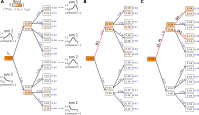
\includegraphics[width=1\textwidth]{Figures/supp/supp1.png}
    \caption{\textbf{Replay updates in Bandit belief space.} A) Planning tree of horizon $2$ constructed by the subject. Each rectangle corresponds to a distinct belief state. The leftmost belief state corresponds to the subject's prior belief, $b_\rho$, at which the tree is rooted. The insets next to some belief states graphically demonstrate the subject's belief about the payoff of one of the arms in those belief states (the red dotted lines show the expected payoffs). For the paired belief states, the top ones always result from imagined successful outcomes (received a reward of $1$), whereas the bottoms ones -- from imagined failed outcomes (received a reward of $0$). Belief states are coloured according to the Need at those belief states calculated by the subject; moreover, Need is additionally shown with numbers in each belief state. Since the subject's behavioural policy is stochastic (softmax), all belief states have positive estimated Need (for some belief states, Need was rounded up to two decimal places). The black arrows show actions available at each belief state. The top arrows always denote the choice of arm $1$ and the bottom ones -- arm $2$. The blue numbers above each action arrow denote the $Q$-values associated with each action in every belief state. B) Single replay update in the belief tree. The subject chose to update the $Q$-value of arm $1$ at the prior belief state (the updated action arrow is highlighted in red) towards the expected value of the two belief states at the next horizon (the new updated value is highlighted in red). This replay update was executed because i) it was estimated to have the greatest EVB; and ii) the estimated EVB of this update exceeded the EVB threshold. Note the effect of generalisation of this individual replay update which is visible in how the Need that the subject calculates for all other belief states changes throughout the tree. C) All replay updates executed by the subject until the estimated benefit was calculated to be below the EVB threshold. The bold numbers in squared brackets show the order in which those updates were executed.}
    \label{fig:supp1}
\end{figure}

\begin{figure}[h!]
    \centering
    \includegraphics[width=1\textwidth]{Figures/supp/supp2.png}
    \caption{\textbf{Policy improvement occasioned by replay.} Top: Evolution of the value of the root belief state (same as in Fig~\ref{fig:supp1}) due to replay as a function of the EVB threhsold, $\xi$. Middle: Evolution of the value of the policy (evaluated in the belief tree) which resulted from replay updates at different EVB thresholds. Bottom: Total number of replay updates executed for the different EVB thresholds.}
    \label{fig:supp2}
\end{figure}

\begin{figure}[h!]
    \centering
    \includegraphics[width=0.9\textwidth]{Figures/supp/supp3.png}
    \caption{\textbf{Effect of initialised behavioural policy}. Top: The final value of the root belief state (same as in Fig~\ref{fig:supp1}) due to replay with a fixed EVB threshold. The initialised values of all belief states were randomised to imitate noisy initial experience (or potential changes in the bandit payoff probabilities). The bars show average root belief state values over $100$ different tree initialisations. Each dot corresponds to an individual tree. Bottom: Same as above but for the value of the updated policy evaluated in the tree.}
    \label{fig:supp3}
\end{figure}

\begin{figure}[h!]
    \centering
    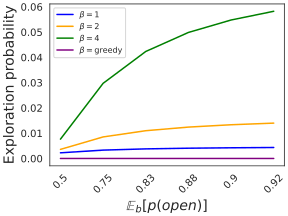
\includegraphics[width=0.9\textwidth]{Figures/supp/supp4.png}
    \caption{\textbf{Sequence replay statistics}. Left: Proportion of forward to reverse sequences replayed in the belief tree with the same prior belief as in Fig~\ref{fig:supp1} with planning horizon set to $4$. The initialised values of all belief states were randomised as in Fig~\ref{fig:supp3}. The bar shows average proportion over $100$ different tree initialisations. Right: Average number of replayed actions in the same tree initialisations as above with and without sequence replay.}
    \label{fig:supp4}
\end{figure}

\begin{figure}[h!]
    \centering
    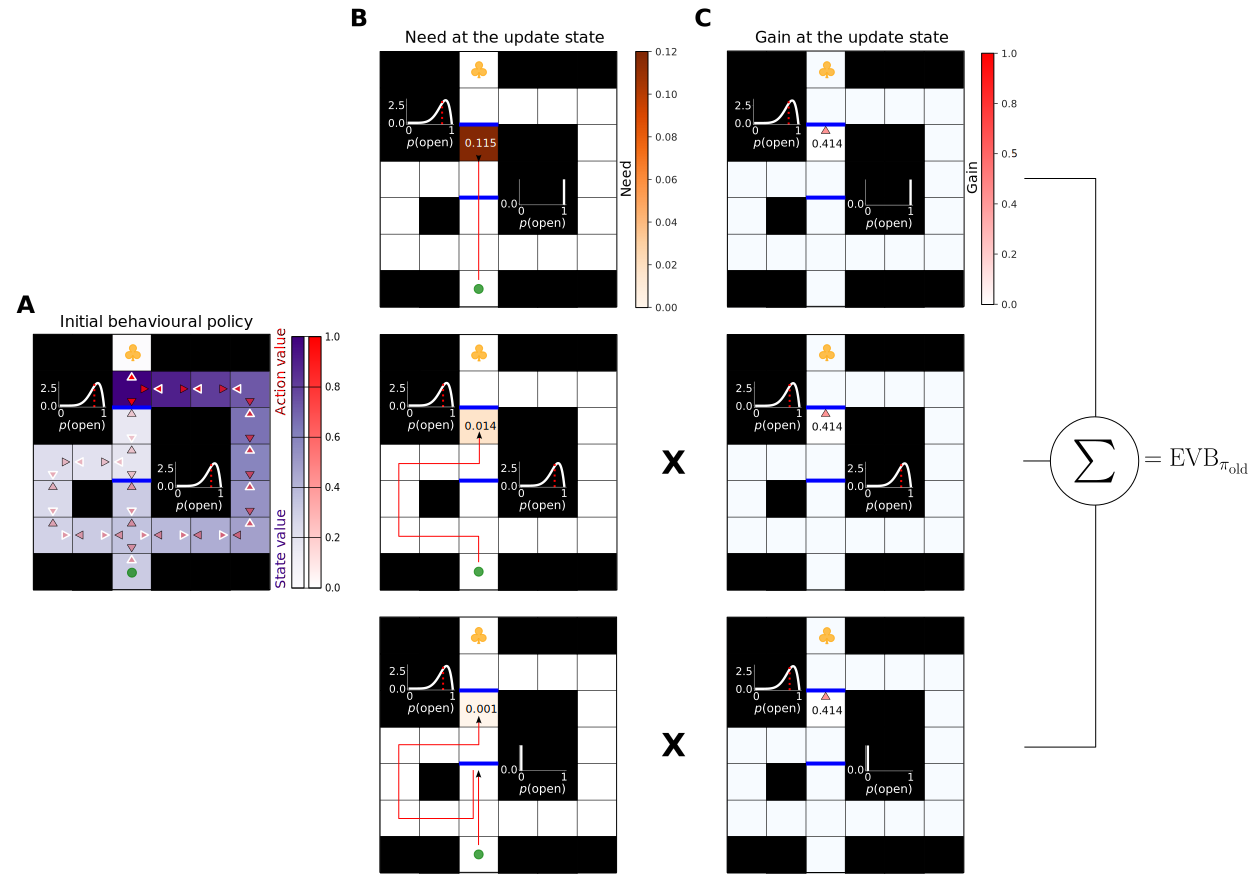
\includegraphics[width=1\textwidth]{Figures/supp/supp5.png}
    \caption{\textbf{Uncertainty affects replay choices and their behavioural readout.} The layout of the figure is similar to that of Fig~\ref{fig:fig3}. A) In this instance, however, the subject's belief was more pessimistic since it indicated a lower chance of the top barrier being potentially open. B) The value of exploration was estimated to be lower, and therefore it did not propagate deep enough (towards the subject's location). C) The updated policy still prescribed the subject to exploit the longer path, since the critical action at the junction between the different arms had not been updated by exploratory replay.}
    \label{fig:supp5}
\end{figure}

\begin{figure}[h!]
    \centering
    \includegraphics[width=0.5\textwidth]{Figures/supp/supp6.png}
    \caption{\textbf{Relationship between uncertainty, behavioural policy and exploration quality.} The graph shows the marginal probability of directed exploration (approaching and attempting the potential barrier in Figs~\ref{fig:fig2} and~\ref{fig:fig3} from the start state) as a function of the subject's uncertainty and the greediness of its behavioural policy. As the subject's belief in the absence of the barrier increased, it became progressively more likely to engage in the act of directed exploration. The same softmax policy with inverse temperature $\beta=2$ was used to calculate the priority of replay updates. However, applying different inverse temperature parameters (which subjects might heuristically use to arrange for offline exploration) to the resulting exploratory value function yielded policies with different incentives for exploration.}
    \label{fig:supp6}
\end{figure}

\clearpage
\printbibliography

\end{document}
